%%---------------------------------------------------------------------------%%
%% NSE Article
%% 2013: RQI+MGE
%%---------------------------------------------------------------------------%%

\documentclass[preprint,12pt]{elsarticle}
%\documentclass[12pt]{article}
\usepackage{amsmath}
\usepackage{amssymb,amsthm,graphicx}
\usepackage{epsfig}
\usepackage[mathcal]{euscript}
%\usepackage{citesort}
\usepackage{setspace}
%\usepackage{tmadd,tmath}
\usepackage{color}
\usepackage{array}
%\usepackage{c++}
%\usepackage{times, mathptm}
\usepackage{subfigure}
%\usepackage{dsfont}

\usepackage{times}
\renewcommand{\ttdefault}{cmtt}

\usepackage{fancyhdr} % used to put page number in header instead of footer

% The float package HAS to load before hyperref
\usepackage{float} % for psuedocode formatting
\usepackage{xspace}
\usepackage{mathrsfs}
\usepackage[pdftex]{hyperref}



%%---------------------------------------------------------------------------%%

%\setlength{\textfloatsep}{8pt plus 1pt minus 1pt}
%\setlength{\abovedisplayskip}{4pt plus 1pt minus 1pt}
%\setlength{\belowdisplayskip}{4pt plus 1pt minus 1pt}
%\addtolength{\oddsidemargin}{-0.5in}
%\addtolength{\textwidth}{1.0in}
%\addtolength{\textheight}{0.5in}

\setlength{\textwidth}{6.5in}
\setlength{\oddsidemargin}{0.0in}
\setlength{\evensidemargin}{0.0in}
\setlength{\textheight}{9.0in}
\setlength{\topmargin}{0.0in}
\setlength{\headheight}{0.0in}
\setlength{\headsep}{0.0in}
\setlength{\footskip}{0.5in}

\renewcommand{\thefootnote}{\fnsymbol{footnote}}
\renewcommand{\thetable}{\Roman{table}}

%%---------------------------------------------------------------------------%%

\newcommand{\email}[1]{$\langle$#1@pitt.edu$\rangle$}

\DeclareMathOperator{\diag}{diag}
\DeclareMathOperator{\low}{lower}
\DeclareMathOperator{\upp}{upper}

\newcommand{\Sn}{\ensuremath{S_N}}
\newcommand{\Macro}{\ensuremath{\Sigma}}

\newcommand{\vOmega}{\ensuremath{\hat{\Omega}}}
\newcommand{\Ye}[2]{\ensuremath{Y^e_{#1}(\vOmega_#2)}}
\newcommand{\Yo}[2]{\ensuremath{Y^o_{#1}(\vOmega_#2)}}

\newcommand{\ve}[1]{\ensuremath{\mathbf{#1}}}

\newcommand{\sigg}[1]{\ensuremath{\sigma^{gg'}_{\text{s}\,#1}}}
\newcommand{\psig}{\ensuremath{\psi^g}}

\newcommand{\even}{\ensuremath{\phi^g}}
\newcommand{\odd}{\ensuremath{\vartheta^g}}

\newcommand{\evenp}{\ensuremath{\phi^{g'}}}
\newcommand{\oddp}{\ensuremath{\vartheta^{g'}}}

\newcommand{\apsi}[1]{\ensuremath{\psi^{\dagger\,#1}}}
\newcommand{\aeven}[1]{\ensuremath{\phi^{\dagger\,#1}}}
\newcommand{\aodd}[1]{\ensuremath{\vartheta^{\dagger\,#1}}}
\newcommand{\asigg}[1]{\ensuremath{\sigma^{g'g}_{\text{s}\,#1}}}

\newcommand{\aPsi}[1]{\ensuremath{\Psi^{\dagger\,#1}}}
\newcommand{\aPhi}[1]{\ensuremath{\Phi^{\dagger\,#1}}}

\newcommand{\epsi}{\ensuremath{\epsilon}}
\newcommand{\ephi}{\ensuremath{\varepsilon}}

\newcommand{\psie}{\ensuremath{\psi_{\epsi}}}
\newcommand{\phie}{\ensuremath{\phi_{\ephi}}}

\newcommand{\Psie}{\ensuremath{\Psi_{\epsi}}}
\newcommand{\Phie}{\ensuremath{\Phi_{\ephi}}}

\newcommand{\apsie}[1]{\ensuremath{\psi^{\dagger\,#1}_{\epsi}}}
\newcommand{\aphie}[1]{\ensuremath{\phi^{\dagger\,#1}_{\ephi}}}

\newcommand{\aPsie}[1]{\ensuremath{\Psi^{\dagger\,#1}_{\epsi}}}
\newcommand{\aPhie}[1]{\ensuremath{\Phi^{\dagger\,#1}_{\ephi}}}

\newcommand{\avg}[1]{\ensuremath{\langle#1\rangle}}

\newcommand{\osig}{\ensuremath{\overline{\sigma}}}
\newcommand{\osigs}{\ensuremath{\overline{\sigma_{\text{s}}}}}

%%---------------------------------------------------------------------------%%

\begin{document}

\setcounter{page}{2}
  
%%---------------------------------------------------------------------------%%

\begin{center}

  {\large \bf Title}
  
  \vspace{0.3in}
  
  R.N. Slaybaugh, T.M. Evans, G.G. Davidson, and P.P.H. Wilson
  
\end{center}

\doublespacing

\vspace{0.3in}

\begin{abstract}

  Abstract

\end{abstract}

\newpage

%%---------------------------------------------------------------------------%%

\section{Introduction}
\label{sec:intro}

A multigrid in energy preconditioner (MGE) that uses a Krylov solver to do the multigroup transport solves has been added to the code Denovo \cite{Evans2010}. This preconditioner compliments the Rayleigh Quotient Iteration (RQI) eigenvalue solver, also available in Denovo. This paper discusses...

%%---------------------------------------------------------------------------%%
\section{Background}
\label{sec:background}
The eigenvalue form of the steady state Boltzmann transport equation is
\begin{align}
   [\hat{\Omega} \cdot \nabla + \Macro(\vec{r}, E)] &\psi(\vec{r}, \hat{\Omega}, E)  = \frac{\chi(E)}{k} \int_0^{\infty} dE' \:\nu \Macro_{f}(\vec{r}, E') \int_{4\pi} d\hat{\Omega'} \:\psi(\vec{r}, \hat{\Omega'}, E') \nonumber \\
   &+ \int_0^{\infty} dE' \int_{4\pi} d\hat{\Omega'} \:\Macro_{s}(\vec{r}, E' \to E, \hat{\Omega'} \cdot \hat{\Omega}) \psi(\vec{r}, \hat{\Omega'}, E') \:,
\label{eq:neutron transport}
\end{align}
%
\noindent where the quantities are at location $\vec{r}$, at energy E, and are traveling in direction $\hat{\Omega}$. The angular neutron flux in neutrons per unit length squared per steradian is $\psi(\vec{r}, \hat{\Omega}, E)$, which expresses the location of the neutrons in phase space; $\Macro_{x}$ is the cross section that represents the likelihood of interaction $x$ (here $s$ is for scattering, $f$ is for fission, and no subscript indicates all interactions) in units of inverse length. Here $\chi(E)$ is the spectrum specifying the energy distribution of neutrons born from fission, $k$ is the asymptotic ratio of the number of neutrons in one
generation to the number in the next, and $\nu$ is the average number of neutrons released per fission. In the fixed source case, the fisission term can be replaced by an external source, $q_{ex}$ \cite{Lewis1993}. 

To numerically solve Equation~\eqref{eq:neutron transport} it is discretized in space, angle, and energy. This work uses the multigroup energy approximation, the scattering term is expanded in Legendre polynomials ($P_l$), and discrete ordinates (\Sn) are used to treat direction of neutron travel. There are many spatial differencing methods available, the discussion of which is beyond the scope of this document as the proposed work is not dependent upon the spatial discretization employed \cite{Evans2009d}. To ensure the new methods apply to the most general cases, it will be assumed that the matrices resulting from discretization are not necessarily symmetric. 

After all of the discretizations are performed, the multigroup \Sn equations can be written in operator form as
%
\begin{alignat}{2}
  \ve{L}\psi &= \ve{MS}\phi + q \:, \qquad &\text{(fixed source)} \label{eq:fxdsource} \\
  \ve{L}\psi &= \ve{MS}\phi + \frac{1}{k}\ve{M}\chi f^{T}\phi \:. \qquad &\text{(eigenvalue)} \label{eq:eigenvalue}
\end{alignat}
%
Here $\ve{L}$ is the first-order linear differential transport operator; $\ve{M}$ is the moment-to-discrete operator that projects the angular flux moments, $\phi$, onto discrete angles; $\ve{S}$ is the scattering matrix; $f$ contains the fission source, $\nu \Macro_{f}$; and $q$ is a source term. The angular flux moments are related to the angular flux through the discrete-to-moment operator: 
\begin{equation}
 \phi = \mathbf{D} \psi \:. \label{eq:disc to mom}
\end{equation}
Using this relationship, Equations \eqref{eq:fxdsource} and \eqref{eq:eigenvalue} can be rearranged such that they are a function of only $\phi$. The formulation is aided by defining $\ve{T} = \ve{DL}^{-1}$ and $\ve{F} = \chi f^{T}$ \cite{Evans2011}:
%
\begin{alignat}{2}
  (\ve{I} - \ve{TMS})\phi &= q \:, \qquad &\text{(fixed source)} \label{eq:OperatorFxdForm} \\
  (\ve{I} - \ve{TMS})\phi &= \frac{1}{k} \ve{TMF} \phi \:. &\text{(eigenvalue)} \label{eq:OperatorEvalForm}
\end{alignat}

Once the matrices are multiplied together, a series of single ``within-group'' equations that are each only a function of space and angle result. If the groups are coupled together by neutrons scattering from a low energy group to a higher energy group, then iterative ``multigroup'' solves over the coupled portion of the energy range may be required. If the eigenvalue is desired, an additional ``eigenvalue'' solve is needed \cite{Evans2009}. Any of these solvers can be accelerated with preconditioning. 

\subsection{Block Krylov Solver}
\label{sec:blockkrylov}
Traditionally, the multigroup solve has been done with Gauss Seidel (GS). GS is iterative in energy. A space-angle solve using a within-group solver, such as source iteration or a Krylov method, is performed for each energy group in series. The groups are solved from $g=0$, the highest energy, to $g=G$, the lowest. For a group $g$ and an energy iteration index $j$ this is \cite{Evans2010}
%
\begin{equation}
  \bigl( \ve{I} - \ve{TMS}_{gg} \bigr) \phi^{j+1}_{g} = \ve{TM} \bigl( \sum_{g'=0}^{g-1}\ve{S}_{gg'}\phi^{j+1}_{g'} + \sum_{g'=g+1}^{G} \ve{S}_{gg'}\phi^{j}_{g'}  + q_{g} \bigr)  \:.
 \label{eq:up-GS}
\end{equation}

The first term on the right includes downscattering contributions from higher energies, and the second term represents upscattering contributions from lower energy groups that have not yet been converged for this energy iteration. Groups that only contain downscattering are simply solved once since the second term on the right is zero. Groups with upscattering, however, must be iterated until they converge. Convergence of GS is governed by the spectral radius of the system, so the method can be very slow when upscattering has a large influence on the solution \cite{Adams2002}. GS is fundamentally serial in energy because of how the group-to-group coupling is treated. 

A recently-added multigroup (MG) Krylov solver removes the traditional \\``within-group'' / ``multigroup'' iteration structure. This allows the solver to handle upscattering efficiently, and enables parallelization in the energy dimension. The solver has been shown to successfully scale to hundreds of thousands of cores. For example, a fixed-source test scaled from 69,102 cores to 190,080 cores with 98\% efficiency \cite{Slaybaugh2011}. 

The MG Krylov solver combines the space-angle and energy iterations to make one space-angle-energy iteration level. This allows the energy groups to be decomposed such that they can be solved in parallel. The space-angle-energy iterations are much like the within-group space-angle iterations, except that the iteration is over a block of groups instead of just one group. The block can include all groups or just upscattering groups, in which case the downscattering groups are treated in series as before. An added benefit of this solver is that Krylov methods generally converge more quickly than GS \cite{Trefethen1997}.

The multigroup Krylov method applied to the upscattering block is shown here, where $\ve{S}_{\text{up\_block}}$ contains the upscattering groups and $\ve{S}_{\text{up\_source}}$ has the downscattering only groups:
%
\begin{equation}
  \underbrace{(\ve{I} - \ve{TMS}_{\text{up\_block}})}_{\tilde{\ve{A}}}\phi_{\text{up\_block}}^{n+1} = \ve{TM}(\ve{S}_{\text{up\_source}}\phi_{\text{up\_source}}^{n+1} + q) \:.
  \label{eq:MGkrylov}
\end{equation}

Trilinos \cite{1089021} provides Denovo's Krylov solver, with a choice of either GMRES or BiCGSTAB \cite{Evans2010}. The Krylov solver is given an operator that implements the action of $\ve{\tilde{A}}$, or the matrix-vector multiply and sweep. In the MG Krylov solver, $\ve{\tilde{A}}$ is applied to an iteration vector, $v$, containing the entire upscattering block instead of just one group:
%
\begin{enumerate}
  \item matrix-vector multiply: $y = \ve{M}\ve{S}_{\text{up\_block}} v$,
  \item sweep: $z = \ve{T} y$,
  \item return: $v \leftarrow v - z$.
\end{enumerate}

To implement the energy parallelization, the problem is divided into energy sets, with groups distributed evenly among sets. After each set performs its part of the matrix-vector multiply, a global reduce-plus-scatter is the only required inter-set communication. Since each set uses the entire spatial mesh with the same spatial decomposition, the established performance of spatial scaling does not change. The space-angle decomposition in Denovo comes from the KBA wavefront algorithm \cite{Baker1998}. Evans et al.\ \cite{Evans2009d} showed scaling in space is limited to about 20,000 cores with a 500 million cell spatial mesh. 

The added energy decomposition offers the ability to further decompose a problem, even if the performance limit of spatial decomposition has been reached. The total number of cores is equal to the number of computational domains, that is, the product of the number of energy sets and the number of spatial blocks. For 20,000 spatial blocks and 10 energy sets, which is a reasonable decomposition, 200,000 cores will be used. See Ref. \cite{Evans2011} for more details. 

The MG Krylov solver makes it possible to use very large machines and fine energy structures. The addition of this solver is one of the key motivators for the MGE preconditioner because Krylov methods often need to be preconditioned to converge in a small number of iterations. A preconditioner that can scale well and handle many energy groups is essential for using the MG Krylov solver. 

\subsection{Eigenvalue Solvers}
\label{sec:eigenvalue}
A common way to solve eigenvalue problems is with PI. This method is attractive because it only requires matrix-vector products and two vectors of storage space. PI uses the form of the problem seen in Eq. \eqref{eq:EnergyDepEval} and then iterates as shown in Eq. \eqref{eq:PowerIteration}, where $i$ is the iteration index. This converts the generalized form of the eigenvalue problem seen in Eq. \eqref{eq:OperatorEvalForm} to the ordinary form. In the generalized form the eigenvector-value pair is $(\phi, \frac{1}{k})$ and in the ordinary form it is $(\phi, k)$. In legacy applications the eigenvector is often the fission source rather than the flux moments \cite{Evans2011}, \cite{Lewis1993}.
\begin{align}
  \ve{A}\phi &= k\phi \:, \label{eq:EnergyDepEval} \\
  \qquad \text{where}  \qquad \ve{A} &= (\ve{I} - \ve{TMS})^{-1} \ve{TMF} \:, \nonumber \\
  \phi^{i+1} = \frac{1}{k^i}\ve{A}\phi^{i} &\:; \qquad 
  k^{i+1} = k^i \frac{f^T \phi^{i+1}}{f^T \phi^i} \:.
  \label{eq:PowerIteration}
\end{align} 
%
Inside of PI, the application of $\ve{A}$ to $\phi$ requires the solution of a multigroup problem that looks like a fixed source problem,
\begin{equation}
  (\ve{I} - \ve{TMS})y^{i} = \ve{TMF}\phi^{i} \:. \label{eq:EvalDepFxdSource}
\end{equation}

PI's convergence can be very slow for problems of interest. For an $n \times n$ matrix $\ve{A}$, an eigenvalue-vector pair satisfies $\ve{A}x_{i} = \lambda_{i}x_{i}$ for $i = 1,...,n$. Let $\sigma(\ve{A}) \equiv \{\lambda \in \mathbb{C} :$\\$ rank(\ve{A} - \lambda \ve{I}) \le n\}$ be the spectrum of $\ve{A}$ and the eigenvalues be ordered as $|\lambda_{1}| > |\lambda_{2}| \ge \dots $\\$\ge |\lambda_{n}| \ge 0$. The error from PI is reduced in each iteration by a factor of $\ve{A}$'s dominance ratio, $\frac{\lambda_{2}}{\lambda_{1}}$. For loosely coupled systems PI will converge slowly because $\lambda_{2}$ is close to $\lambda_{1}$ \cite{Trefethen1997}. 

Shifted inverse iteration (SII) typically converges more quickly than PI. SII capitalizes on the fact that for some shift $\mu$, $(\ve{A} - \mu \ve{I})$ will have the same eigenvectors as $\ve{A}$. If $\mu \notin \sigma(\ve{A})$, then $(\ve{A} - \mu \ve{I})$ is invertible and $\sigma([\ve{A} - \mu \ve{I}]^{-1}) = \{1/(\lambda - \mu):\lambda \in \sigma(\ve{A})\}$. Eigenvalues of $\ve{A}$ that are near the shift will be transformed to extremal eigenvalues that are well separated from the others. The shifted and inverted matrix is used in a power iteration-type scheme. Given a good shift, $\mu \approx \lambda_1$, SII usually converges more quickly than PI, especially for loosely coupled systems \cite{Trefethen1997}, \cite{Allen2002}.

Wielandt's method is a flavor of SII that has been used widely in the neutron transport community %, though it was originally developed in 1944 in an unrelated context 
\cite{Zinzani2008}, \cite{Itagaki1996}, \cite{Itagaki2002}. In the transport equation formulation, Wielandt's method changes the eigenvalue problem to $(\ve{I} - \ve{TM}(\ve{S} +\gamma_e \ve{F}))\phi = \delta \gamma \ve{TMF} \phi$, where $\gamma_e$ is the current estimate for the dominant eigenvalue, $\gamma_1 = \frac{1}{k}$, and $\delta \gamma = \gamma_1 - \gamma_e$. The power method is applied to this, giving \cite{Nakamura1977}
%
\begin{equation}
\phi^{i+1} = \delta \gamma^{i}(\ve{I} - \ve{TM}(\ve{S} + \gamma_e \ve{F}))^{-1}\ve{TMF}\phi^{i} \:. \label{eq:Wielandt}
\end{equation}

Rayleigh Quotient Iteration is a shifted inverse iteration method that uses an optimal shift. RQI applies a shift to the equations via the scattering matrix in a manner similar to Wielandt's method. This can cause some complications for common fixed source solvers.

The scattering matrix is lower triangular for groups that have downscattering. There are entries above the diagonal only when there is upscattering. The fission matrix has an energy-block filled column for every group with fission. Applying the shift as $(\ve{S} + \gamma_e \ve{F})$ makes the scattering matrix energy-block dense even when there is very little upscattering. Traditional solution methods for the fixed source part of the equation do not handle dense scattering matrices well. This has hampered the implementation of SII in multi-group, 3-D codes because solving many groups that have upper-triangular scattering entries will take a long time. To overcome this barrier, a new solver is needed. 

RQI has been implemented in Denovo by subtracting $\rho \ve{TMF}$ from both sides of %$(\ve{I} - \ve{TMS})\phi =$ \\ $\gamma \ve{TMF}\phi$. 
Eq. \eqref{eq:OperatorEvalForm}. This gives the following shifted system where $\gamma \equiv \frac{1}{k}$:
%
\begin{align}
  (\ve{I} - \ve{TM}\ve{\tilde{S}})\phi &=( \gamma - \rho) \ve{TMF} \phi  \:, 
  \label{eq:OperatorShiftedEval} \\
  \text{ where } \ve{\tilde{S}} &\equiv \ve{S} + \rho\ve{F}  \nonumber \:.
\end{align}
%
The new matrix, $\ve{\tilde{S}}$, is energy-block dense since the fission matrix is dense. $\ve{\tilde{S}}$ looks like one big upscattering block and can be treated similarly. By using the new MG Krylov solver over all groups the entire problem can be decomposed in energy and solved efficiently. Note that using GS to solve a problem with a dense $\tilde{\ve{S}}$ would likely take a very long time to converge. More details about RQI in Denovo can be found in Ref.\ \cite{Slaybaugh2012}.

\subsection{Multigrid in Energy Preconditioner}
\label{sec:precond}
For many kinds of problems the total number of multigroup iterations required to adequately converge the transport equation is large. To reduce iteration count, a preconditioner can be applied to transform the system of interest into another equivalent system that has more favorable properties and is easier to solve. 
 
Right preconditioning leaves the right hand side of the equation unaffected and does not change the norm of the residual, which is used for convergence testing in most iterative methods. Right preconditioning is therefore often preferred over left or split preconditioning for iterative solvers \cite{Knoll2004}. A right preconditioner was implemented in this work, and the remaining discussion will be presented in right preconditioner format. 

Let $\ve{G}$ be a non-singular preconditioner. Then $\ve{A}x=b$ can be transformed as 
%
\begin{equation}
  \ve{AG}^{-1}y = b, \qquad  x = \ve{G}^{-1}y \:.
\end{equation}
%
The matrix $\ve{A}\ve{G}^{-1}$ is not formed in practice. The preconditioner can be applied by using some method to solve $\ve{G}y=c \to y \approx \ve{G}^{-1}c$, or by otherwise implementing the action of $\ve{G}^{-1}$ without explicitly forming and inverting $\ve{G}$ \cite{Benzi2002}.

Preconditioning is important for increasing the robustness of Krylov methods. This is particularly true for the multigroup Krylov solver. This solver can create large Krylov subspaces because it forms the subspaces with multiple-group-sized vectors. As a result, any reduction in iteration count will have a significant benefit in terms of memory and cost per iteration. Prior to this work, there was no preconditioner in Denovo that could work with the MG Krylov solver. 

The new preconditioner does multigrid in the energy dimension. To understand why multigrid in energy makes sense for neutron transport, some highlights about these methods are discussed here. See \emph{A Multigrid Tutorial} by Briggs, Henson, and McCormick~\cite{Briggs2000} for a thorough and approachable explanation of what multigrid methods are and why they work.

The error in $x_i$, the $i$th guess for $\ve{A}x_i=b_i$, can be written as a combination of Fourier modes. Each Fourier mode has a frequency, and the frequencies can range from low-frequency (smooth) to high-frequency (oscillatory). Iterative methods, also referred to as smoothers or relaxers, remove high-frequency error components quickly, but take many iterations to remove the low-frequency ones. 

The idea of multigrid methods is to take advantage of the smoothing effects of iterative methods by making smooth errors look oscillatory and thus easier to remove. Errors that are low-frequency on a fine grid can be mapped onto a coarser grid where they are high-frequency. A relaxer is applied on the coarser grid to remove the now oscillatory error components. The remaining error is mapped to a still coarser grid and smoothed again. The problem is restricted to coarser and coarser grids until it is on a grid which is coarse enough to directly invert the equations.

Next, the coarsest result is prolonged back to the next-finer grid and used to correct the solution there. A few relaxations are done on this finer grid. The errors are prolonged back up the chain, continuously correcting on finer grids, until the finest grid is reached. This entire process is called a V-cycle. 

Multigrid methods are differentiated by how many times the V-cycle is done and how many grids are used. The optimal combination of grids and cycles may depend on problem type. The addition of more grids and cycles will reduce error, but at an added cost.
 
A multigrid method was selected for many reasons. Multigrid methods remove the low-frequency error modes that require many Krylov iterations. The preconditioner was designed to take advantage of the energy decomposition used by the MG Krylov method. Each energy set can do work on its own grids and does not need to communicate with other energy sets. This is a communication savings compared to using grids in space or angle. An additional benefit is the simplicity of energy grids. Energy is one-dimensional, which allows for simpler coarsening and refinement than spatial or angular grids.

Recall that \\$\ve{A} = \ve{I} - \ve{TMS}$. To implement this in Denovo, $y$ is defined as $\ve{G}\phi$ and the problem is broken into two steps: 
%
\begin{enumerate}
  \item with a Krylov method solve 
    \begin{equation}
      \ve{AG}^{-1}y = b \:, \label{eq:PrecondKrylov} 
    \end{equation}
  \item after finding $y$, calculate 
    \begin{equation}
      \phi = \ve{G}^{-1}y \:. \label{eq:PrecondPhi}
    \end{equation}
\end{enumerate}

To build energy grids, the energy group structure is coarsened so that each lower grid has fewer groups. The finest grid is the input energy structure, and the coarsest grid has one or a few groups. Each level has half as many groups as the previous level, rounded up if applicable. If there are $G+1$ groups on the fine grid there will be either $\frac{G+1}{2}$ or $\frac{G+2}{2}$ groups on the coarse grid. This is conceptually straightforward because the energy groups can be combined (restricted) and separated (prolonged) linearly.

The implemented restriction operator is a simple averaging scheme. Neighboring fine data are averaged together to make coarse data. To prolong from a coarse to a fine grid, the points that line up between the grids are mapped directly. To fill in the intermediate points on the fine grid, the adjacent coarse values are averaged. There are other restriction and prolongation operators that are more rigorous and would preserve more accuracy when transferring between grids than those implemented. For example, a full weighting restriction operator would be more rigorous in combination with the current prolongation method than the current restriction operator is \cite{Briggs2000}.

The user chooses the number of V-cycles done for each preconditioner application. One V-cycle proceeds from the finest grid to the coarsest grid and back to the finest. The input option specifies the number of V-cycles that are concatenated together, with a default of 2. Each additional V-cycle should remove more error, but has a computational cost. 

The depth of the V-cycle can also be specified by the user. The default behavior is determined by the number of groups, such that the grids will be coarsened until there is only one energy group. The number of grids needed is given by \cite{BinaryTree2012}
\begin{equation}
  \text{floor}\bigl( \log_{2}(G-1) \bigr) + 2 \:.
  \label{eq:NumGrids}
\end{equation}
%
How this is handled when using energy sets is discussed below. 

Some number of relaxations are performed on each level while traversing down and up the grids in a V-cycle. The number of relaxations per level is a user input choice with a default of 2. Performing more relaxations per grid should remove more error, but has a computational cost. The implemented relaxation method is weighted Richardson iteration. When applied to the transport equation, we obtain
%
\begin{equation}
  \phi^{m} = \bigr(\ve{I} + \omega(\ve{TMS} - \ve{I})\bigl)\phi^{m-1} + \omega b^{m-1} \:,
  \label{eq:relax}
 \end{equation}
%
where $\omega$ is a constant selected by the user that defaults to 1. 

An important principle is that the preconditioner is only attempting to approximately invert $\ve{A}$. It is therefore reasonable to use a less accurate angular discretization in the preconditioner than the rest of the code. For example, the whole problem may be solved at $S_{10}$, but the preconditioner could only use $S_{2}$. There is an input option to specify an angular quadrature set to use in the preconditioner different from the angular quadrature set used in the rest of the problem; the default is to use the same set in both. At this time, this option has only been implemented for vacuum boundary conditions. 

The other approach is to prohibit cross-set communication by having each set do its own ``mini'' V-cycle. Each set restricts, prolongs, and relaxes on only its own groups. This strategy requires there to be at least two groups on every set. With an unequal number of groups per set, there is a choice between forcing all sets to have the same grid depth or allowing those with more groups to have deeper Vs. The first option enforces energy load balancing between sets, while the second allows the sets with more groups to remove more error. 

The preconditioner is implemented so that all sets use the same grid depth. The benefit of load balancing is likely to be greater than having some sets use an extra grid. Thus, each set restricts to one or two group(s), giving approximately $num\_sets$ total groups across all sets at the coarsest level. The number of grids needed is determined by the set with the minimum number of groups, since it will be the first to reach a grid with one group. This modifies Equation~\eqref{eq:NumGrids} to be
\begin{align}
  num\_g_{min} &= \text{floor}\bigl(\frac{num\_groups}{num\_sets}\bigr) \:, \\
  num\_grids &= \text{floor}\bigl( \log_{2}(num\_g_{min}) \bigr) + 2 \:.
  \label{eq:multisetGrids}
\end{align}

The communication costs and logistical complications of the first strategy seem likely to overwhelm the benefit gained by going to one group instead of $num\_sets$ groups. The second strategy was chosen because it involves much less communication and overhead cost. The value of this choice will become apparent in the results section. 

With the implemented energy set strategy, there are trade-offs between the number of sets and the number of grids for a fixed number of groups. When there are more sets, more cores can be used at once and wall time should decrease. When there are fewer sets each V-cycle can go deeper, so the preconditioner should be more effective at reducing iteration count.  


%%---------------------------------------------------------------------------%%
\section{Past Work}
This section is a high-level summary of past work in the field and a brief summary of results from the MGE Preconditioner used with fixed source problems or PI, and from unpreconditioned RQI.

\subsection{Unpreconditioned RQI}
(Physor Paper)
\begin{enumerate}
 \item RQI works as well as PI from a time and iteration count perspective for very simple problems
 \item With an itermediately sized problem RQI got close to the correct $k$, but failed to converge
 \item RQI did not converge at all on 2D and 3D C5G7 benchmarks: demonstrated need for preconditioning
\end{enumerate}

\subsection{MGE Preconditioner}
(JCP MGE paper)
\begin{enumerate}
 \item established r, v, w choice guidance w/ small fixed source problem
 \item demonstrated that using a reduced angle set inside the preconditioner is very valuable with FeC cube
 \item FeC problem used to show very good energy scaling behavior when full grid-depth is chosen 
 \item FeC problem also used to who that using a reduced grid depth is just as beneficial as full grid depth (likely makes energy scaling less impressive)
 \item 3D C5G7 benchmark with PI showed MGE greatly reduced iteration count, but not computation time
 \item full PWR also showed fewer iterations, but preconditioned PI took way longer than unpreconditioned PI
\end{enumerate}


%%---------------------------------------------------------------------------%%
\section{Results}
%Introductory sentence about studying whether RQI is possible when used with MGE. The preconditioning parameters are the Richardson iteration weight, $w_{k}$, the number of V-cycles per preconditioner application, and the number of relaxations per level. 

%The syntax used throughout this section will be that $w\#$ is the weight, $r\#$ is the number of relaxations per level, and $v\#$ is the number of V-cycles, e.g.\ $w1r1v1$ is one relaxation per level, one V-cycle, and a weight of 1. Using more preconditioning means using larger values of $w$ and/or $r$ and/or $v$. Other issues investigated are changing the depth of the V-cycle, using a different quadrature set inside the preconditioner than in the rest of the problem, and strong scaling. 

%The goal of using the preconditioner is to improve convergence behavior of the multigroup Krylov solves. The best metric for measuring this is the total number of multigroup Krylov iterations used in a calculation because it is the most consistent and fair measure. The number of eigenvalue iterations is also compared for the eigenvalue tests. This is a point of interest rather than a measure of goal attainment. The total number of Krylov iterations is the best proxy for convergence behavior as it encompasses the work that is done within each eigenvalue iteration.  

%Timing comparisons should be considered heuristically unless otherwise specified. In cases where the calculations were done on a single core, the machine was not dedicated to these calculations and times could vary if the same calculations were repeated. Some problems use an optimized version of the code and others use a debug version. These should give the same iteration count, but not necessarily the same relative times between problems. Further, little effort has been made to optimize the preconditioner for speed. Once the multigrid in energy preconditioner has been optimized for efficiency, the preconditioned times should decrease. How much improvement can be gained is a matter for future study. 

%Unless otherwise noted, all test problems used a step characteristic spatial solver, level-symmetric angular quadrature, and the grid depth was determined using the default approach, Equation~\eqref{eq:NumGrids} or Equation~\eqref{eq:multisetGrids}. The Krylov solver was GMRES, which is set to limit the number of multigroup iterations to 1,000 if the problem does not converge earlier. The convergence tolerances are noted for each problem. The tolerance for the multigroup solve is the convergence tolerance used by GMRES in Trilinos \cite{1089021}. The eigenvalue tolerance is used by PI to determine if the eigenvalue has converged. In Denovo, PI also checks the L2-norm and the infinity-norm of the difference in the fission source between iterations. The default L2-norm tolerance is 1.0 and infinity-norm tolerance is 0.01.

\subsection{RQI+MGE Results from Thesis}
\subsubsection{Parameter and Shifted precond Investigation}
** Can probably leave this out, or leave out shifted data (maybe discuss in a paragraph why it's a bad idea and state studies showed this) **\\
vacuum unshifted: base parameter guidance\\
vacuum shifted: fewer iterations, sometimes incorrect answer\\
reflecting unshifted: more parameter guidance, a bit different from vacuum\\
reflecting shifted: bad news

\subsubsection{Intermediate problem}
RQI kinda choked on this without preconditioning, but behaved really really poorly with preconditioning. This was the one with negative fluxes and complete crazy behavior that we never explained. Worked fine with MGE+PI. Worked worse with BiCGSTAB instead of GMRES. 

\begin{table}[!h]
\caption{Infinite Medium Eigenvalue Problem, Preconditioning Results with Rayleigh Quotient Iteration}
\begin{center}
\begin{tabular}{| c | c | c | c | l | c | c | c | c |}
\hline
$w$ & $r$ & $v$ & $k$ & Krylov & RQI & Max Rel Diff & RMS Err & Rel Time$^{+}$ \\[0.5ex]
\hline
0    & 0 & 0 & 0.3970 & 39,025              & 40$^{*}$  & n/a & n/a & 211.03 \\%$5.43 \times 10^{4}$ \\
1    & 1 & 1 & 0.3982 & 3,014$^{\dag}$ & 4 & $1.67 \times 10^{-1}$ & $3.32 \times 10^{-2}$ & 103.56 \\%$2.66 \times 10^{4}$ \\
1    & 3 & 1 & 0.3983 & 50                     & 3 & 0.0 & 0.0 & 40.19 \\ %$1.03 \times 10^{4}$ \\
1    & 4 & 1 & 0.3983 & 44$^{\dag}$      & 3 & 0.0 & 0.0 & 4.51 \\ %$1.16 \times 10^{3}$ \\
1    & 2 & 2 & 0.3983 & 44$^{\dag}$      & 3 & 0.0 & 0.0 & 1.11 \\ %$2.86 \times 10^{2}$ \\
1    & 4 & 4 & 0.4001 & 16                     & 3 & $1.67 \times 10^{-1}$ & $3.21 \times 10^{-2}$ & 7.73 \\ %$1.99 \times 10^{3}$ \\
1    & 5 & 4 & 0.4001 & 14$^{\dag}$     & 3 & $1.67 \times 10^{-1}$ & $3.21 \times 10^{-2}$ & 8.81 \\ %$2.27 \times 10^{2}$ \\
1.4 & 5 & 4 & -0.4711 & 12$^{\dag}$    & 2 & $1.67 \times 10^{-1}$ & $3.21 \times 10^{-2}$ & 6.77 \\ %$1.74 \times 10^{3}$ \\
1    & 5 & 5 & -0.4575 & 7$^{\dag}$      & 2 & $3.43 \times 10^{-6}$ & $3.67 \times 10^{-5}$ & 6.13 \\ %$1.58 \times 10^{3}$ \\
\hline
1.1 & 4 & 1 & 0.3983 & 43$^{\dag}$      & 3 & 0.0 & 0.0 & 4.51 \\ %$1.16 \times 10^{3}$ \\
1.1 & 1 & 4 & 0.3983 & 43$^{\dag}$      & 3 & 0.0 & 0.0 & 5.24 \\ %$1.35 \times 10^{3}$ \\
1.1 & 2 & 2 & 0.3983 & 43$^{\dag}$      & 3 & 0.0 & 0.0 & 4.57 \\ %$1.18 \times 10^{3}$ \\
\hline
0.7 & 1 & 1 & 0.3999 & 3,001$^{\dag}$ & 4 & 1.0 & $3.72 \times 10^{-1}$ & 87.34 \\ %$2.25 \times 10^{4}$ \\
0.7 & 3 & 1 & 0.4001 & 87$^{\dag}$      & 5 & 0.0 & 0.0 & 7.60 \\ %$1.95 \times 10^{3}$ \\
0.7 & 3 & 3 & 0.4001 & 47$^{\dag}$      & 5 & 0.0 & 0.0 & 11.34 \\ %$2.92 \times 10^{3}$ \\
0.4 & 3 & 1 & 0.4001 & 1,052$^{\dag}$ & 4 & $1.18 \times 10^{-5}$ & $8.43 \times 10^{-8}$      & 67.57 \\ %$1.74 \times 10^{4}$ \\
\hline 
\end{tabular}\\
$^{+}$compared to unpreconditioned PI, $2.57 \times 10^{2}$ seconds\\
$^{*}$terminated manually\\
$^{\dag}$negative flux
\end{center}
\label{table:impi RQI}
\end{table}
%
The preconditioned results are shown in Table~\ref{table:impi RQI}. In the table ``Max Rel Diff'' is the maximum over all cells and all groups of the relative difference between the reference flux and the absolute value of the computed flux, $\max[ (\phi_{ref} - \vert\phi_{calc}\vert) / \phi_{ref}]$. ``RMS Err'' is the root mean squared (rms) relative error, $\sqrt{ \sum_{1}^{N}(rel\_err)^{2} / N}$. As a reminder, the total and upscattering tolerances were $1 \times 10^{-4}$, and the $k$ tolerance was $1 \times 10^{-5}$. Recall that if the Krylov iteration count is in the thousands it means the eigenvector did not converge in every iteration. The ``Rel Time'' column is the ratio of the found time to the unpreconditioned PI time of $2.57 \times 10^{-2}$ seconds.

** Should we leave this out?\\
** Should we try to understand this better?\\
** Is it unethical to leave out this data?\\

\subsubsection{2D C5G7}
%Next, the preconditioner was applied to the 2-D C5G7 benchmark using both PI and RQI with the goals of seeing if preconditioned RQI could converge the flux and $k$, to investigate the effect of preconditioning in both RQI and PI, and to see whether the lessons learned about preconditioning parameters still hold in a real problem. The calculation used 16 cores on the small orthanc cluster at Oak Ridge: 4 $x$-blocks, 4 $y$-blocks, 1 $z$-block and 1 energy set. The total and upscattering tolerances were $1 \times 10^{-3}$, with a $k$ tolerance of $1 \times 10^{-5}$. An optimized version of Denovo was used.  

A weight variation study was done with power iteration first. The results using $r1v1$ are plotted as Krylov Iterations vs.\ Weight, and Time in seconds vs.\ Weight in Figure~\ref{fig:2-Dc5g7PI}. The data that is plotted can be found in Appendix~\ref{sec:AppendixD}, Table~\ref{table:2-D c5g7}. All calculated $k$s were within the uncertainty of the benchmark and so are not reported. All preconditioned cases needed 31 power iterations while the unpreconditioned case took 32.
%
\begin{figure}[!ht]
    \begin{center}
      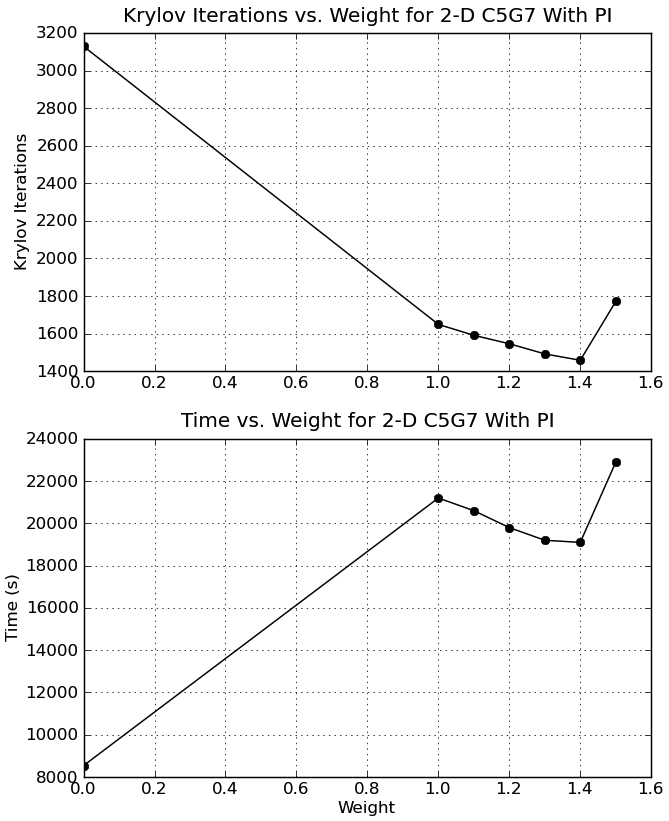
\includegraphics [width=0.7\textwidth, height=0.7\textheight] {2Dc5g7PI}
   \end{center}
   \caption{2-D C5G7 Benchmark, Preconditioner Weight Variation with Power Iteration}
   \label{fig:2-Dc5g7PI}
\end{figure}

%This study shows the preconditioner is very effective at reducing the number of Krylov iterations used by power iteration. The unpreconditioned case, corresponding to a weight of 0 on the plot, took 3,129 MG Krylov iterations. As the weight was increased from 1 to 1.4, the number of Krylov iterations and the time to solution both decreased. With $w1.4$, 1,458 MG Krylovs were taken. The time and iteration count both went back up with a weight of 1.5. When the weight was increased beyond 1.5 none of the multigroup iterations converged, and the problem was terminated manually after several power iterations. 

Two other calculations with a higher level of preconditioning were also done. When the parameters were $w1.4r2v2$ the number of Krylov iterations were reduced to 438 and the calculation took $1.77 \times 10^{4}$ seconds, both lower than all the cases using $r1v1$. For $w1r3v3$, 253 Krylov iterations and $2.28 \times 10^{4}$ seconds were required. This had the smallest number of Krylov iterations, but a slightly longer time than all the calculations except $w1.5r1v1$.	

%The results from the RQI study are in Table~\ref{table:2-D c5g7 rqi}. In all cases, except the unpreconditioned one, $k$ was within the uncertainty of the benchmark value. The ``$<$ 1,000?'' column indicates whether or not the multigroup iterations converged during the RQI process. If the value is ``no'' that means the eigenvector only converged during the first iteration. A number indicates the last eigenvalue iteration for which the Krylov method took less than 1,000 iterations. All subsequent iterations required the full 1,000. A ``yes'' means all of the Krylov iterations converged. The relative time is the ratio of the case of interest to the unpreconditioned PI time of $8.54 \times 10^{3}$ seconds.
%
\begin{table}[!h]
\caption{2-D C5G7 Benchmark, Convergence Study with Rayleigh Quotient Iteration}
\begin{center}
\begin{tabular}{| c | c | c | l | c | c | c |}
\hline
Weight & Relaxations & V-cycles & Krylov & RQI & $<$ 1,000? & Rel Time$^{\dag}$\\[0.5ex]
\hline
0    & 0 & 0 & 119,006 & 120$^{*}$ & no & 10.98 \\%$9.38 \times 10^{4}$ \\
1    & 1 & 1 & 16,007   & 17            & no & 23.65 \\ %$2.02 \times 10^{5}$ \\
1.2 & 1 & 1 & 40,008   & 41$^{*}$   & no & 13.00 \\ %$2.06 \times 10^{5}$ \\
1    & 3 & 1 & n/a         & n/a$^{*}$  & 7   & n/a \\
1    & 2 & 2 & 11,158   & 19            & alternated & 46.72 \\ %$3.99 \times 10^{5}$ \\
1    & 3 & 2 & 3,320     & 19            & 14 &19.23 \\ % $1.64 \times 10^{5}$ \\
\hline
1    & 3 & 3 & 299        & 19            & yes & 3.01 \\ %$2.57 \times 10^{4}$ \\
1.1 & 3 & 3 & 281        & 19            & yes & 2.80 \\ %$2.40 \times 10^{4}$ \\
1.3 & 3 & 3 & 254        & 19            & yes & 2.57 \\ %$2.19 \times 10^{4}$ \\
1.5 & 3 & 3 & n/a         & n/a$^{*}$ & no & n/a \\
\hline 
\end{tabular} \\
$^{\dag}$compared to unpreconditioned PI, $8.54 \times 10^{3}$ seconds\\
$^{*}$terminated manually
\end{center}
\label{table:2-D c5g7 rqi}
\end{table}
%

%These results show a few important things. Most significantly, with enough preconditioning the multigroup iterations within RQI can be converged and the right eigenpair can be found. For the first three $w\#r3v3$ cases all of the Krylov iterations converged. In these cases the calculation time decreased by an order of magnitude compared to the ones where they did not converge every time because so many fewer eigenvalue iterations were needed. This test case was the first to demonstrate that the preconditioner can get RQI to converge. 

%For many of the calculations the eigenvector did not converge or did not converge all the time, but the correct eigenvalue was still found (even in the $w1.2r1v1$ case that was terminated manually). As the preconditioning increased, the eigenvector came closer to converging for all iterations. When the Krylov iterations converged, increasing the weight decreased iteration count and wall time for small weights. As in other tests, too much weight caused the calculation not to converge at all. 

%Additionally, it seems that preconditioning held RQI on track enough to get the right eigenvalue when the eigenvector did not quite converge. As was hypothesized for the unpreconditioned infinite medium test, it may be that the eigenvector was close enough to correct that a good approximation to the eigenvalue could still be made from it, even though the vector itself did not converge. 

Only the $w1r3v3$ calculation overlaped between RQI and PI. PI took fewer Krylov iterations, 253 compared to 299, and less time, $2.28 \times 10^{4}$ compared to $2.57 \times 10^{4}$ seconds. For this test preconditioned RQI did not perform as well as preconditioned PI, though the times and iteration counts were close to one another. 

%From the standpoint of comparing eigenvalue solution methods, it is worth noting that RQI required 19 eigenvalue iterations while PI required 31. Both methods use eigenvectors from the inside multigroup solves to compute eigenvalues in the outer iterations. When given eigenvectors that have been converged to the same tolerance, RQI needed fewer eigenvalue iterations than PI. In this case it took more Krylov iterations within each multigroup solve to get the eigenvector to that tolerance, so RQI was not better in terms of total Krylov count.

The RQI problem was also tried with BiCGSTAB as the Krylov solver for an unpreconditioned case and a $w1r3v3$ case. Every multigroup iteration went to the 1,000 iteration limit and the problem was terminated manually after several RQ iterations.

\subsubsection{3D C5G7}
%The preconditioner using both PI and RQI was also applied to the 3-D C5G7 benchmark with an optimized version of Denovo. The goals of this study were essentially the same as the 2-D study, except that this problem is larger, and the first to approach a real ``grand challenge'' type of calculation. The medium-sized oic cluster at Oak Ridge was used and each problem was given 720 cores with 40 $x$-blocks, 18 $y$-blocks, and 5 $z$-blocks. The total and upscattering tolerances were $1 \times 10^{-4}$, with a $k$ tolerance of $1 \times 10^{-5}$ unless otherwise indicated. The wall time limit was 12 hours. 

%The power iteration results are in Table~\ref{table:3-D c5g7}. The relative time is compared to unpreconditioned PI, $4.46 \times 10^{3}$ seconds. The unpreconditioned power iteration calculation computed a $k$ that was not within the uncertainty bounds of the reported benchmark; it was low by about 0.011. All preconditioned PI and RQI tests computed a $k$ that was within the Denovo $k$ tolerance of the unpreconditioned PI result so they are not reported here. Subsequent to these calculations it was determined that using a more accurate quadrature gives the correct $k$. 
%
%\begin{table}[!h]
%\caption{3-D C5G7 Benchmark, Preconditioning Parameter Scoping with Power Iteration}
%\begin{center}
%\begin{tabular}{| c | c | c | c | l | c |}
%\hline
%Weight & Relaxations & V-cycles & Krylov & PI & Rel Time$^{\dag}$ \\[0.5ex]
%\hline
%0    & 0 & 0 & 1,224 & 32 & 1.00 \\ %$4.46 \times 10^{3}$ \\
%1    & 1 & 1 & 708    & 32 & 5.90 \\ %$2.12 \times 10^{4}$ \\
%1.2 & 1 & 2 & 448    & 32 & 5.33 \\ %$2.38 \times 10^{4}$ \\
%1.2 & 2 & 1 & 448    & 32 & 5.37 \\ %$2.39 \times 10^{4}$ \\
%1.3 & 2 & 2 & 288    & 32 & 6.37 \\ %$2.84 \times 10^{4}$ \\
%1    & 3 & 3 & 126    & 14$^{*}$  & 9.05 \\ %$4.04 \times 10^{4}$ \\
%1.5 & 3 & 3 & 192    & 32 & 8.36 \\ %$3.73 \times 10^{4}$ \\
%1    & 4 & 4 & n/a     & n/a          & exceeded wall time \\
%1    & 4 & 4 & n/a     & n/a$^{*}$ & exceeded wall time \\
%1.5 & 5 & 5 & n/a     & n/a          & exceeded wall time \\
%\hline 
%\end{tabular}\\
%$^{\dag}$compared to unpreconditioned PI, $4.46 \times 10^{3}$ seconds\\
%$^{*}$tol and upscatter tol = $1 \times 10^{-5}$, $k$ tol = $1 \times 10^{-3}$
%\end{center}
%\label{table:3-D c5g7}
%\end{table}

%The 3-D benchmark study shows the preconditioner with PI can reduce the number of required Krylov iterations substantially for challenging problems. The number of eigenvalue iterations for a given tolerance set were never changed by preconditioning. 

%The effect of preconditioning parameters was consistent with what was observed in other test problems. However, using large values for $r$ and $v$ made the calculation take too long to get results. On the oic machine, if a calculation exceeds wall time there is no way to get any of the results from the scratch space. Therefore, no conclusions can be drawn from this problem about the effect of substantial preconditioning when using power iteration for a real, 3-D problem. 

The RQI results are in Table~\ref{table:3-D c5g7 rqi}. The relative time is compared to unpreconditioned PI, $4.46 \times 10^{3}$ seconds. Many cases did not finish in time to report results. What is likely happening when the problems with lower parameter values run out of time is that the eigenvector is not converging. As was seen before, the calculations take a long time when every eigenvalue iteration uses 1,000 Krylov iterations. Unfortunately, there is no way to confirm this theory or find out if the eigenvalue is close to correct since the output cannot be obtained. 
%
\begin{table}[!h]
\caption{3-D C5G7 Benchmark, Preconditioning Parameter Scoping with Rayleigh Quotient Iteration}
\begin{center}
\begin{tabular}{| c | c | c | c | l | c |}
\hline
Weight & Relaxations & V-cycles & Krylov & RQI & Rel Time$^{+}$ \\[0.5ex]
\hline
0    & 0 & 0 & n/a     & n/a          & exceeded wall time \\
1    & 1 & 1 & n/a     & n/a          & exceeded wall time \\
1.5 & 1 & 1 & n/a     & n/a          & exceeded wall time \\
1.2 & 2 & 1 & n/a     & n/a          & exceeded wall time \\
1.3 & 2 & 2 & 302    & 19           & 5.20 \\ %$2.32 \times 10^{4}$ \\
1    & 3 & 3 & 103    & 9$^{*}$    & 6.67 \\ %$3.02 \times 10^{4}$ \\
1    & 3 & 3 & 164    & 15$^{\dag}$ & 7.59 \\ %$3.38 \times 10^{4}$ \\
1.5 & 3 & 3 & 187    & 19           & 7.26 \\ %$3.24 \times 10^{4}$ \\
1    & 4 & 4 & n/a     & n/a          & exceeded wall time \\
1    & 4 & 4 & 74     & 9$^{*}$    & 5.13 \\ %$2.29 \times 10^{4}$ \\
1.5 & 5 & 5 & n/a     & n/a          & exceeded wall time \\
\hline 
\end{tabular}\\
$^{+}$compared to unpreconditioned PI, $4.46 \times 10^{3}$ seconds\\
$^{*}$tol and upscatter tol = $1 \times 10^{-5}$, $k$ tol = $1 \times 10^{-3}$\\
$^{\dag}$tol and upscatter tol = $1 \times 10^{-4}$, $k$ tol = $5 \times 10^{-5}$
\end{center}
\label{table:3-D c5g7 rqi}
\end{table}  

With an intermediate amount of preconditioning, RQI converged and performed better than the analogous PI cases. There are three cases where both problems finish and the same tolerances were used: $w1.3r2v2$, $w1r3v3$, $w1.5r3v3$. These results are shown together in Table~\ref{table:PI RQI} for ease of comparison. This table displays time instead of relative time since the comparison is between two cases rather than across all cases. In all three the RQI calculations took less time and fewer eigenvalue iterations than PI. In the second two they also took fewer Krylov iterations. RQI even finished in time to get results from the $w1r4v4$ calculation when PI did not. 
%
\begin{table}[!h]
\caption{3-D C5G7 Benchmark, Rayleigh Quotient Iteration and Power Iteration Comparison}
\begin{center}
\begin{tabular}{| c | c | c | c | c | c | c |}
\hline
Sovler & Weight & Relaxations & V-cycles & Krylov & Eigenvalue & Time (s) \\[0.5ex]
\hline
RQI & 1.3 & 2 & 2 & 302    & 19           & $2.32 \times 10^{4}$ \\
PI    & 1.3 & 2 & 2 & 288    & 32           & $2.84 \times 10^{4}$ \\
\hline
RQI & 1    & 3 & 3 & 103    & 9$^{*}$   & $3.02 \times 10^{4}$ \\
PI    & 1    & 3 & 3 & 126    & 14$^{*}$ & $4.04 \times 10^{4}$ \\
\hline
RQI & 1.5 & 3 & 3 & 187    & 19           & $3.24 \times 10^{4}$ \\
PI    & 1.5 & 3 & 3 & 192    & 32           & $3.73 \times 10^{4}$ \\
\hline 
\end{tabular}\\
$^{*}$tol and upscatter tol = $1 \times 10^{-5}$, $k$ tol = $1 \times 10^{-3}$
\end{center}
\label{table:PI RQI}
\end{table}  

%The 3-D benchmark problem shows that for at least some problems, preconditioned RQI converges more quickly in all senses than preconditioned PI. It is pertinent that this is true is the most interesting problem shown so far. It seems, however, that RQI can only be useful if it is preconditioned enough to get the eigenvector to converge. 

%These results continue to confirm that a small amount of weight works well for real problems. Increasing $r$ and $v$ decrease iteration count, but at what can be a high time penalty. An intermediate amount of preconditioning will likely provide the best balance of reduced iteration count for the time invested once the preconditioner is optimized. 

** Could do more of these with better w,r,v choices to have more overlap between RQI and POI; use reduced angle set; not much grid depth to reduce, but could try anyway **

\subsection{PWR 900 new results}
Most cases: tolerance = 1e-3, L2 tolerance = 1e-3, k tolerance = 1e-3. 578 x 578 x 700 cells (233,858,800 cells), 112 x 112 x 10 partitions (12,544 blocks). $S_{12}$, P0, 44 groups. 1.73 trillion unknowns. k0 = 1. Depth of V-cycle = 2, \Sn  in MGE = $S_2$
%
\begin{table}[!h]
\caption{PWR-900 Comparison of PI and RQI with and without preconditioning on 11 energy sets}
\label{tab:PWR all}
  \begin{center}
    \begin{tabular}{| c | c | c | c | c | c | c |}
      \hline
      Method & Precond & N Eigen & N Krylov & k & time (m) \\\hline
      %%
      RQI & none   & info &     &                     & \\
      RQI & w1r1v1 & 3   & 45   & 1.252 $\pm$ 1.13e-2 & 120$^*$ \\
      RQI & w1r2v2 & 5   & 70   & 1.268 $\pm$ 9.75e-4 & 54.8 \\
      PI  & none   & 149 & 5602 & 1.276 $\pm$ 4.34e-6 & 612.2 \\
      PI  & w1r1v1 & info &     &                     & \\
      PI  & w1r2v2 & 86  & 946  & 1.275 $\pm$ 1.43e-5 & 720$^*$ \\
      \hline
      PI  & none   & 24  & 901  & 1.272 $\pm$ 1.01e-4 & 92.1$^\dagger$ \\
      PI  & w1r1v1 & info &     &                     & \#$^\dagger$\\
      PI  & w1r2v2 & 28  & 312  & 1.273 $\pm$ 8.24e-5 & 250.9$^\dagger$ \\
      \hline
    \end{tabular}\\
    $^{*}$did not converge within walltime limit\\
    $^{\dagger}$tolerance = $1 \times 10^{-2}$, $k$ tolerance = $1 \times 10^{-2}$
  \end{center}
\end{table}

\begin{table}[!h]
\caption{PWR-900 RQI strong scaling w1r2v2 preconditioning}
\label{tab:PWR rqi strong scaling}
  \begin{center}
    \begin{tabular}{| c | c | c | c | c | c | c |}
     \hline
      Sets & N Eigen & N Krylov & time (m) & t$_{\text{perfect}}$ & Efficiency \\\hline
      %%
      1   & 5 & 70 & 407.8 & 407.8 & 1.000 \\
      4   & 5 & 70 & 123.4 & 102.0 & 0.826\\
      11  & 5 & 70 & 54.8  & 37.1  & 0.676\\
      22  & 5 & 70 & 39.6  & 18.5  & 0.468\\
      \hline
    \end{tabular}
  \end{center}
\end{table}

With a lower tolerance also have: \\
1) a strong scaling study \\
2) one reduced angle set comparison

%%---------------------------------------------------------------------------%%

\section{Conclusions}
\label{sec:conclusions}

Conclusions

%%---------------------------------------------------------------------------%%

\section{Acknowledgements}

This research used resources of the Oak Ridge Leadership Computing Facility at the Oak Ridge National Laboratory, which is supported by the Office of Science of the U.S. Department of Energy under Contract No. DE-AC05-00OR22725. Additional thanks to the Rickover Fellowship Program in Nuclear Engineering sponsored by Naval Reactors Division of the U.S. Department of Energy. This fellowship sponsored the work from which this work is derived. 

%%---------------------------------------------------------------------------%%

\newpage
\appendix

\section{Angular Flux Moments}
\label{sec:angular-flux-moments}

Appendix

%%---------------------------------------------------------------------------%%
%% BIBLIOGRAPHY
%%---------------------------------------------------------------------------%%

\newpage

\singlespacing

\bibliographystyle{model1-num-names}
\bibliography{RQI_MGE}

%%---------------------------------------------------------------------------%%
%% TABLES
%%---------------------------------------------------------------------------%%

\clearpage

\begin{table}[p]
  \caption{
    Comparison of results for the adjoint neutron porosity tool
    problem. For these problems, the adjoint source is place in the
    far detector.  All timing results are normalized to the
    unaccelerated Gauss-Seidel iteration time.
  }
  \label{tab:adjoint-porosity-tool}
  \begin{center}
    \begin{tabular}{lcll}\hline\hline
      Method & Acceleration $S_N$ order & GS iterations & Time \\\hline
      %%
      GS & - & 53 & 1.0   \\
      TTG & 8 & 7 & 0.172 \\
      TTG & 2 & 7 & 0.159 \\
      \hline\hline
    \end{tabular}
  \end{center}
\end{table}

%%---------------------------------------------------------------------------%%

\clearpage

\begin{table}[p]
  \caption{
    Results from the neutron porosity tool problem using MTTG.  All
    timing results are normalized to the unaccelerated Gauss-Seidel
    iteration time.
  }
  \label{tab:MTTG-porosity-tool}
  \begin{center}
    \begin{tabular}{llllll}\hline\hline
      Method & Acceleration $S_N$  & GS Iterations & Within-group
      & Acceleration & Time \\
      & order & & sweeps & sweeps &  \\\hline
      %%
      GS   & - & 175 & 16294 & 0    & 1.0   \\
      TTG  & 8 & 15  & 1398  & 547  & 0.113 \\
      TTG  & 2 & 13  & 1212  & 459  & 0.086 \\
      MTTG & 2 & 47  & 611   & 1329 & 0.050 \\
      \hline\hline
    \end{tabular}
  \end{center}
\end{table}

%%---------------------------------------------------------------------------%%
%% FIGURES
%%---------------------------------------------------------------------------%%

\clearpage

\begin{figure}[p]
  \begin{center}
    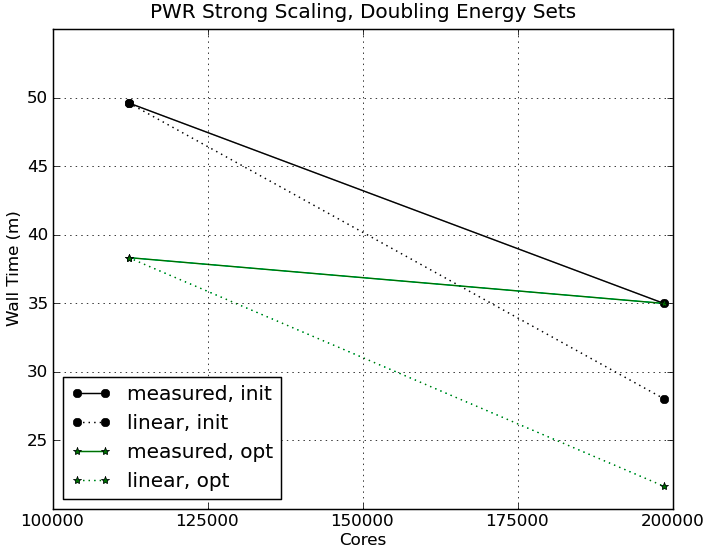
\includegraphics[width=6in,clip]{PWRstrongScaling}
  \end{center}
  \caption{Example1}
  \label{fig:example1}
\end{figure}

%%---------------------------------------------------------------------------%%

\clearpage

\begin{figure}[p]
  \begin{center}
    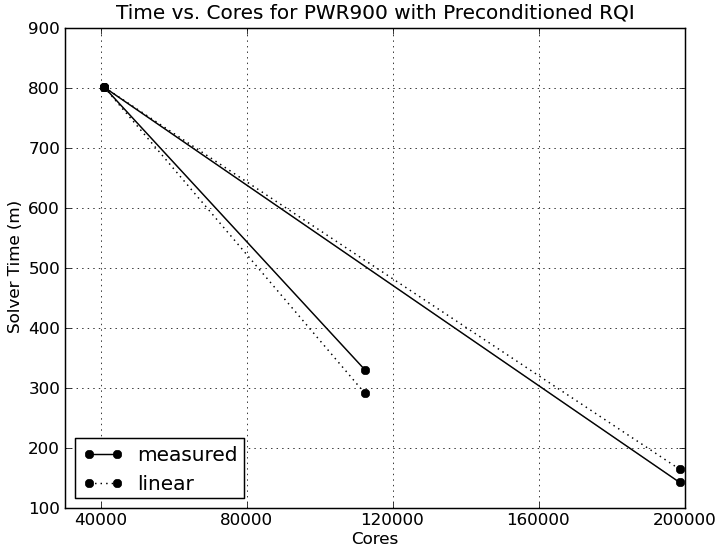
\includegraphics[width=6in,clip]{PWRPrecondRQI}
  \end{center}
  \caption{Example}
  \label{fig:example2}
\end{figure}

%%---------------------------------------------------------------------------%%

\clearpage

\singlespacing
\begin{center}

  {\Large \bf Title}
  
  \vspace{0.3in}
  
  {\large R.N. Slaybaugh\footnote{Corresponding author.  Telephone: +1
      570 850 3385.  E-mail: rns37@pitt.edu.}\\
    Department of Mechanical Engineering and Material Science\\
    University of Pittsburgh\\
    605 Benedum Hall, 3700 O'Hara Street\\
    Pittsburgh, PA 15261, USA\\\vspace{1\baselineskip}
    T.M. Evans, G.G. Davidson\\
    Radiation Transport and Criticality Group\\ 
    Oak Ridge National Laboratory\\ 
    P.O. Box 2008\\
    Oak Ridge, TN 37831-6170, USA\\\vspace{1\baselineskip}
    P.P.H. Wilson\\
    Department of Nuclear Engineering and Engineering Physics\\
    University of Wisconsin - Madison\\
    419 ERB, 1500 Engineering Drive\\
    Madison, WI 52706, USA\\}
  
  \addtocounter{page}{-1}

  \vspace{2.0in}
  \renewcommand{\thetable}{\arabic{table}}
  \thepage\ Pages --- \thetable\ Tables --- \thefigure\ Figures \\

  \setcounter{page}{1}

\end{center}

%%---------------------------------------------------------------------------%%

\end{document}

%%---------------------------------------------------------------------------%%
%% end of paper.tex
%%---------------------------------------------------------------------------%%
